\chapter{Generation}
\ifpdf
    \graphicspath{{Management/ManagementFigs/PNG/}{Management/ManagementFigs/PDF/}{Management/ManagementFigs/}}
\else
    \graphicspath{{Management/ManagementFigs/EPS/}{Management/ManagementFigs/}}
\fi

The final stage of development involves generating new, novel and creative poetry by utilising the information gathered in the previous analysis and interpretation sections.

\section{Approach}
Most previous attempts at automatic poetry generation, including ones mentioned in Section \ref{sec:related_work}, prioritise adherence to poetic features and structure above all else. This is done with the justification that:
\begin{itemize}
\item{poetry rarely follows syntactical rules of English grammar.}
\item{readers of poems, as humans, are extremely apt at finding subtle meaning in language, even if it was not intended by the author.}
\end{itemize}

Veale argues that 'poetic licence' is not a licence but a contract that allows a speaker to take liberties in language in exchange for real insight\cite{veale2013less}. We are in support of Veale's argument that grammatical rules in poetry are only broken for \textit{some purpose} like matching a rhyme scheme or rhythm pattern. They are broken with precision and intention, not arbitrarily or randomly.

Furthermore, we discussed in Section \ref{sec:semantics} that even grammatically correct sentences can be completely nonsensical. We require understanding of the semantic relationships between words to be able to write with intention and in a way that can be understood by the reader. As discussed in Section \ref{sec:purpose}, the purpose of poetry is to deliver a specific, intentional message. This cannot be done without control over language both syntactically and semantically.

Therefore, our approach will be \textbf{content first}. We aim to produce poetry that follow syntax and semantics as far as possible and only make specific exceptions for the sake of poetic features.

Finally, this implementation should be able to produce any type of poem in accordance with the information gathered in the analysis and interpretation. We cannot make any assumptions on the length of the lines, the existence of rhyme or the topics covered by the poems.


%~~~~~~~~~~~~~~~~~~~~~~~~~~~~~~~~~~~~~~~~~~~~~~~~~~~~~~~~~~~~~~~~~~~~~~~~~~~~~~~~~~~~~~~~~~~~~~~~~~~~~~
\section{Generating Simple Sentences}
\label{sec:build}
We attempted to recognise the existence of semantic relations during the analysis phase. Our interpretation of the results generalises the use of these relations with the intention of guiding the generation process. If we intend to write a poem describing a woman named Mary who wants a monkey, we would start with the persona relation hubs in Figure \ref{fig:starting}.
\begin{figure}[h!]
\centering
\begin{subfigure}[t]{0.45\textwidth}
	\centering
    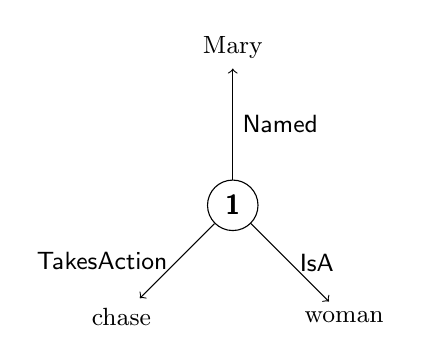
\begin{tikzpicture}[->, node distance=2cm,main node/.style={circle, draw, font=\sffamily\bfseries}]
        \tikzstyle{every node}=[font=\small]
        
          \node[main node] (1) [] {1};
          \node[] (3) [above of=1]{Mary};
          \node[] (4) [below right of=1] {woman};
          \node[] (5) [below left of=1] {chase};
          
        
          \path[every node/.style={font=\sffamily\small}]
            (1) edge node [right] {Named} (3)
               	edge node [right] {IsA} (4)
               	edge node [left] {TakesAction} (5);
              
        \end{tikzpicture}
    \caption{First persona}
\end{subfigure}
~
\begin{subfigure}[t]{0.45\textwidth}
	\centering
    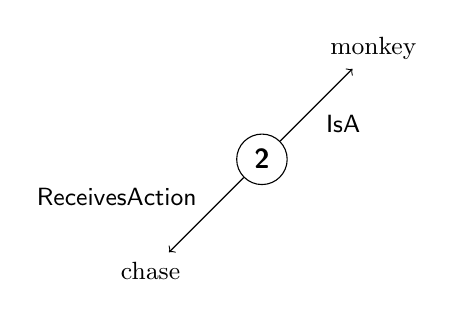
\begin{tikzpicture}[->, node distance=2cm,main node/.style={circle, draw, font=\sffamily\bfseries}]
        \tikzstyle{every node}=[font=\small]
        
          \node[main node] (1) [] {2};
          \node[] (3) [above right of=1]{monkey};
          \node[] (4) [below left of=1] {chase};
          
        
          \path[every node/.style={font=\sffamily\small}]
            (1) edge node [below right] {IsA} (3)
               	edge node [above left] {ReceivesAction} (4);
              
        \end{tikzpicture}
    \caption{Second Persona}
\end{subfigure}
\caption{Starting relations for generation}
\label{fig:starting}
\end{figure}

These relations outline the context of the poem. In lieu with our \textit{content first} approach, we begin by directly translating these relations into syntactically correct natural language \textit{clauses}, which can be organised into lines in a poem. We make use of two tools to do this; \textbf{SimpleNLG} (Section \ref{sec:bg-nlg}) and \textbf{FrameNet} (Section \ref{sec:fn}).

We choose to use SimpleNLG because it provides an almost bespoke interface into the features of the sentence that we picked out in the analysis stage, allowing us to apply the results directly to our new poems.

These features include:
\begin{itemize}
\item{Tense}
\item{Aspect}
\item{Perspective}
\item{Negation}
\item{Animation, Gender, Plurality}
\item{Determiners}
\end{itemize}

\subsection{Translating Relations into Clauses}
We used FrameNet when deriving relations with SEMAFOR in Section \ref{sec:chars} by checking for the existence of certain frames. Now we reverse the process; use selected frames that correspond to particular relations to define the type and roles of phrases during generation.

Take the Desire relation for example. The corresponding frame in FrameNet would be \textit{Desiring}. The general translation process follows this algorithm:

\begin{verbatim}
1 look up LUs from given Frames/IDs/Word
2 select a Valence Pattern
3 order phrases in Valence Pattern so that subjects come first, then the target, then the dependencies and objects
4 fill in the phrases with relevant words
\end{verbatim}

Suppose we take the \textit{1-Named$\rightarrow$Mary} relation in Figure BLAH above. We have a character whose ID is 1 and has the name 'Mary'. The corresponding frame for the 'Named' relation is \textit{Referring\_by\_name}. 

However, it is not quite a perfect match because we only want verbs, whereas this frame includes Lexical Units (LUs) of other parts of speech as well. Each LU gives indication of its part-of-speech (POS) so we can filter by that. 

Another complication is that the verb 'to name' does not exist in the FrameNet lexicon at all. The closest match is the adjective 'named' found in the \textit{Being\_named} frame. So we need to be able to look up this LU manually as well.

Yet another issue is that not all of these LUs come with full and accurate Valence patterns. FrameNet is an ongoing project with more data being added continuously so we do not want to use a word that does not have an accurate set of Valence patterns. Thankfully, the status of every LU is provided, so we only look up those that have the \textit{Finished\_Initial} annotation.

It is important to note that all relation translations may have their own set of similar caveats that are to be considered on a case by case basis to improve the quality of lines generated. Furthermore, while the TakesAction and ReceivesAction phrases enable us to use any verb in the FrameNet lexicon, having specific builder algorithms for as many relations as possible will greatly increase the quality and variation of language capabilities.

Back to our example, after dealing with all issues we are left with two LUs; \textit{call.v} and \textit{named.a}, where the string after the full stop in the LU indicates the word's POS. We choose one randomly with equal weights. We use \textit{call.v} for this example.

\begin{table}
    \begin{tabular}{|llll|}
    \hline
    Number Annotated & Pattern part 1 & Pattern part 1 & Pattern part 1 \\ \hline
    19 TOTAL         & Entity         & Name           & ~              \\
    (1)              & CNI,--        & NP,Obj        & ~              \\
    (1)              & NP,Ext        & AVP,Dep       & ~              \\
    (11)             & NP,Ext        & NP,Dep        & ~              \\
    (6)              & NP,Ext        & NP,Obj        & ~              \\ \hline
    16 TOTAL         & Entity         & Name           & Speaker        \\
    (1)              & NP,Ext        & NP,Dep        & CNI,--        \\
    (1)              & NP,Ext        & NP,Obj        & CNI,--        \\
    (1)              & NP,Ext        & PP[by],Dep    & CNI,--        \\
    (5)              & NP,Obj        & NP,Dep        & NP,Ext        \\
    (1)              & NP,Obj        & PP[by],Dep    & CNI,--        \\
    (5)              & NP,Obj        & PP[by],Dep    & NP,Ext        \\
    (2)              & NP,Obj        & QUO,Dep       & NP,Ext        \\ \hline
    1 TOTAL          & Name           & Name           & ~              \\
    (1)              & NP,Dep        & NP,Ext        & ~              \\ \hline
    \end{tabular}
\caption{Valence patterns for the \textit{call.v} LU}
\label{tab:call-val}
\end{table}

This LU has three groups of Valence patterns, as can been seen in Table \ref{tab:call-val}. Each group of patterns has an \textit{TOTAL} count, indicating the occurrence frequency of this pattern in their annotated corpus. We assume that these are representative for our purpose and choose the group with the highest total occurrences.

Each pattern within a group also includes an occurrence count. However, the phrases produced by the system would be predictable and mundane if we always choose the most popular again. Instead we select randomly, weighted for occurrence scores. Let our selected Valence pattern be the third one from the top in Figure BLAH.

We then order the phrases according to how they would appear in a sentence; subjects first (\textit{Ext}), then the target word, followed by the dependencies (\textit{Dep}) and objects (\textit{Obj}).

The Valence pattern does not include the LU itself so we add it as a verb phrase immediately after the subject.

Finally, we fill in the gaps by adding carefully selected words to each phrase. We discuss word selection in Sections  \ref{sec:persona} and \ref{sec:new-lines}.

%~~~~~~~~~~~~~~~~~~~~~~~~~~~~~~~~~~~~~~~~~~~~~~~~~~~~~~~~~~~~~~~~~~~~~~~~~~~~~~~~~~~~~~~~~~~~~~~~~~~~~~
%~~~~~~~~~~~~~~~~~~~~~~~~~~~~~~~~~~~~~~~~~~~~~~~~~~~~~~~~~~~~~~~~~~~~~~~~~~~~~~~~~~~~~~~~~~~~~~~~~~~~~~
\subsection{Semantic Network of Common Sense}
\label{sec:common-sense}
We discussed the idea of modelling the mind as a search space by connecting related concepts together in a network in Section \ref{sec:common-sense-bg}. We gathered inspiration from ConceptNet and discussed Tom De Smedt's attempt to model creativity with such a construct.
 
We aim to replicate the experiment bespoke to our purposes, outlined in this section.
 
\subsubsection{The Network}
The primary purpose of our network is to help us build clauses out of one or two words. For this, we require our semantic network to give indications of \textbf{actions} that nouns take and receive, as well as \textbf{properties} they have.

The secondary purpose of the network is to provide associative data so to maintain a cohesive topic flow through the poem, rather than jumping between a variety of topics. 

\paragraph{Nodes}
As with previous attempts, the nodes of the network are the \textit{concepts}, represented by words. We take a step further by enriching these nodes with the POS of the word so to disambiguate between different meanings (e.g. \textit{bear} the noun and \textit{bear} the verb).

\paragraph{Edges}
The edges of the network indicate the relationship between concepts. They are \textit{directed} in our graph. The types of edges are:
\begin{description}
\item[HasProperty] \hfill \\ Stereotypical descriptions of the head of the relation. \hfill \\ doctor.n - HasProperty $\rightarrow$ smart.a \hfill \\ run.v - HasProperty $\rightarrow$ quickly.adv
\item[IsA] \hfill \\ Taxonomy of the head of the relation (hypernymy). \hfill \\ E.g. banana.n - IsA $\rightarrow$ fruit.n
\item[PartOf] \hfill \\ The head of the relation is typically a constituent or member of the tail.  \hfill \\ finger.n - PartOf $\rightarrow$ hand.n
\item[TakesAction] \hfill \\The head of the relation typically performs the action in the tail. \hfill \\ lion.n - TakesAction $\rightarrow$ roar.v
\item[ReceivesAction] \hfill \\The head of the relation typically has the action in the tail done unto it. \hfill \\ book.n - ReceivesAction $\rightarrow$ read.v
\item[RelatedTo] \hfill \\ Any non-specific, reversible association. \hfill \\ fat.a - RelatedTo $\rightarrow$ eat.v \hfill \\ eat.v - RelatedTo $\rightarrow$ food.n \hfill \\ food.n $\rightarrow$ RelatedTo
\end{description}

All edges are of equal weight at this stage. There is potential for prioritising certain types of relations or concepts to bias the vocabulary. For example, we could weight scientific words higher than regular ones to make the program lean towards a more advanced vocabulary.


\paragraph{Concept Halos and Fields}

The Concept Halo and Field work in the same way as described in Section  \ref{sec:common-sense-bg}. We use them to fill in the gaps in the sentence with intelligent word selection. For example, if we are given a verb, we can lookup the concept field for that verb looking only at TakesAction and ReceivesAction edges to find possible subjects and objects for the verb. Similarly, we can find modifiers for verbs and nouns by looking up HasProperty edges their respective concept halos.

\subsubsection{Sources}
There are various sources for semantic relationships between words. Some are more applicable to our use case given the nature of relations that we desire and the quality of the source.

\paragraph{Collocations}
The Oxford Collocations Dictionary, as described in Section \ref{sec:ox-colloc}, provides the set of words and POS commonly occur in relation to any given word.

The dictionary entry for \textit{custard} can be seen in Figure \ref{fig:custard-collocs-2}. It gives common adjectives that are used to describe custard, which can be converted into \textit{HasProperty} relations. It also shows that custard receives the action of being made, poured and strained, while it takes the actions of thickening and setting. Furthermore, we can infer that it is closely related to \textit{powder} and \textit{pie}.

\begin{figure}[h!]
\centering
\includegraphics[width=140mm]{custard-collocs}
\caption{Oxford Collocations Dictionary entry for \textit{'custard'}}
\label{fig:custard-collocs-2}
\end{figure}

We can extract relations directly by parsing this dictionary, which is freely available in compressed HTML format. As the dictionary is developed by Oxford and is used by students of English, its entries are very high quality and dependable.

\paragraph{Associations}
We discussed The University of South Florida Free Associated Norms in Section \ref{sec:fl-assoc}, which provides general associations between words. It continues to be used for research and is therefore another source that can be depended on for quality as it was collected in a scientifically sound manner.

The POS of each word is provided but no direction in the association can be determined. Therefore, we may be able to assume that a noun has the property of an associated adjective and that an adjective is a property of associated nouns. However, we cannot assume the whether a noun takes or receives the action of an associated verb. Therefore we use the more general \textit{RelatedTo} relationship instead.

\paragraph{NodeBox Perception}
The NodeBox Perception model, as discussed in section \ref{sec:nb-percep}, has plenty of overlap in the types of semantic relations used in Perception as we will be using for this project, including 'is-a' (\textit{IsA}), 'is-property-of' (reversed HasProperty), 'is-part-of' (\textit{PartOf}) and 'is-related-to' (\textit{RelatedTo}). We generalise all other relations to our \textit{RelatedTo} relation.

This data was manually entered into the system and continues to be used for research, which means that it is a high-quality source of data.

\paragraph{WordNet}
\ref{sec:wn}
As mentioned in Section, WordNet is very large and already has fast and simple interfaces from Python, so we do not merge its meronym (\textit{PartOf}), hypernym and holonym (\textit{IsA}) relations with our knowledge graph at this point. While it may prove useful to consolidate all data in a single graph in the future, it is not necessary at this stage as we can still benefit fully from its data without doing so.

\paragraph{Google Search Suggestions}
While we currently do not preprocess relations in the way Veale did to produce Metaphor Magnet (see Section \ref{sec:goog-sugg}), we do use a similar method to help complete sentences, particularly those with indirect objects. 

For example, we would be able to produce a sentence like \textit{'Mary hit the nail with'} but be unable to complete the sentence due to a lack of information of indirect objects. However, Google suggestions auto-complete \textit{'hit the nail with'} with \textit{'hammer'}, as one might expect. 

This is the least dependable source of information that we use, so we only use it for that specific case and do not add any to our knowledge network.


\subsubsection{Concept Similarity}
Similarity between concepts in the knowledge network is the primary method of guiding word choice throughout the poem. We deal with two main types of similarity; associative and symbolic.

\paragraph{Associative Similarity}
\label{sec:assoc-sim}
Associative similarity between concepts is represented by the length of the shortest past between them in our network. We use Dijkstra's Algorithm\cite{dijkstra1959note} as the underlying implementation of our shortest path algorithm.

Associative similarity helps us choose the best replacement word from a list of candidates. This is very useful when rephrasing to match rhyme and rhythm and will be explained in greater detail in Section \ref{sec:rephrase}. 

It can also help us choose applicable words to start new lines of poetry that stay within context (see Section \ref{sec:inc-growth}).

In both of these cases, we are finding the \textit{most} similar concept from a list of candidates of unknown length. The brute force implementation can quickly increase both space and memory complexity. To fix this, we alter Dijkstra's Algorithm to have a limited search depth. This way, if we know the shortest path to one of the candidates is $x$, we can abort any further searches that go beyond length $x$ for the shortest path.

\paragraph{Similarity Paths}
Paths from one concept do more than show the extent of the relationship - they also show intermediary concepts taken to get from one to the other. This can be a powerful way of joining two concepts together that may not be on consecutive lines.

For example, suppose the first line of a poem mentions the concept \textit{'man.n'} and the third line \textit{'myth.n'} (Section \ref{sec:apply-inspr} explains how this scenario might arise). The path in the knowledge network between these two concepts goes via the concept \textit{'mystery.n'}, which we can use to seed the second line creating a smooth topic flow through the poem.


\paragraph{Symbolic Similarity}
Symbolic similarity can be attained through inductive reasoning and substitution by concepts that have a very similar concept halo and field up to a certain depth. Simply put, we can find similarity with the \textit{Duck Test}: if it looks like a duck, swims like a duck and quacks like a duck, it probably is a duck. Object-oriented programmers can relate this idea to the Liskov substitution principle.

Symbolic similarity has many use cases, including the new method of anaphora resolution to be proposed for future work. For this phase, it enables us to implement the following poetic features:
\begin{description}
\item[Similes] \hfill \\ We can describe a property or an action of a persona in our poem by comparing the persona to an concept in our knowledge network that (stereotypically) has that property or takes/receives that action. \hfill \\ The relation \textit{1- TakesAction $\rightarrow$ run quickly} can be built into the phrase 'runs like a cheetah' by recognising that cheetahs are stereotypically quick runners.
\item[Metaphors] \hfill \\ Similarly to Similes, we can find concepts in our network that share a number of semantic relations with the persona we are trying to describe. \hfill \\ Any persona with relations \textit{1 - TakesAction $\rightarrow$ crawl}, \textit{1 - HasProperty $\rightarrow$ social} and \textit{1 - HasProperty $\rightarrow$ small} is analogous to an insect because its concept in the graph shares those relations.
\item[Personification] \hfill \\ If we are given an inanimate object as a persona, we can describe it as if it were sentient by looking giving it relations that belong to a sentient being. \hfill \\ A car could be personified by giving it all the relations that a lion has in our concept network, to produce sentences like \textit{'The car roared'}.
\item[Irony] \hfill \\ Our knowledge network is made up of semantic attributes that are expected for each concept. Irony can be attained by producing lines of poetry that describe a concept doing the opposite of the concepts given in our graph.
\end{description}
%~~~~~~~~~~~~~~~~~~~~~~~~~~~~~~~~~~~~~~~~~~~~~~~~~~~~~~~~~~~~~~~~~~~~~~~~~~~~~~~~~~~~~~~~~~~~~~~~~~~~~~
%~~~~~~~~~~~~~~~~~~~~~~~~~~~~~~~~~~~~~~~~~~~~~~~~~~~~~~~~~~~~~~~~~~~~~~~~~~~~~~~~~~~~~~~~~~~~~~~~~~~~~~

\section{Persona Creation and Management}
\label{sec:persona}
\subsection{Referencing Specific Persona}
When we convert the relation \textit{1-Named$\rightarrow$Mary} in Figure BLAH to a phrase, we need to refer to the persona using \textit{IsA} relations. The clause will be built with the verb 'named' and object 'Mary', and we look up the persona that this relation was taken from and find an \textit{IsA} relation to use as the subject. In this example, we will find \textit{'woman'} and when we add the determiner \textit{'a'}, we get the clause \textit{'a woman named Mary'}.

We follow a similar process when converting the \textit{1-TA$\rightarrow$chase} relation. The only difference is now that we can use the name of the persona as another candidate for the subject. This will give us either \textit{'The woman chases'} or \textit{'Mary chases'}.

\subsection{Adding New Persona}
The verb 'chase' is \textit{transitive}, i.e. it requires a subject \textbf{and} an object, so we need a persona that receives the action 'chase'. If we look through the relations of the other known persona, we will find the relation \textit{2-RA$\rightarrow$chase} and we use \textit{2-IsA$\rightarrow$monkey} to derive the corresponding reference to that character. We complete the sentence by adding \textit{'monkey'} to the end, giving us either \textit{'The woman chases a monkey'} or \textit{'Mary chases a monkey'}.

Suppose we could not find a corresponding ReceivesAction relation for 'chase' in any of the current set of persona. We must then find a concept in our knowledge network that receives the action 'chase' to use as the object of the clause. We do this by looking at the concept field of the \textit{'chase.v'} concept in our knowledge graph for only the edges with type ReceivesAction. This gives us the required list of concepts from which to select the object of the clause. We use concept similarity to find the most applicable object given the current context of the poem; a process to be described in detail in Section \ref{sec:new-lines}, but for now let's assume that we use the concept \textit{'thief.n'}.

When we add a new noun to the poem, we need to create a new persona object so that we can refer back to it later. The new character is instantiated with an IsA relation to its noun word, i.e. \textit{thief}. Its plurality, gender and animation are all derived from the word itself using the process described in Section \ref{sec:characters}.

\subsection{Anaphora and Presupposition}
So far we are only able to refer to persona by \textit{Named} or \textit{IsA} relations that are already part of the persona's hub. This leads to to combinations of clauses such as \textit{'There was a woman named Mary. Mary chased the monkey'}, which is not natural speech.

The natural way to phrase it could be \textit{'There was a woman named Mary. She chased the monkey'}. In this case, the introduction of the pronoun 'she' is a contextual reference back to the aforementioned persona. This is introduction of anaphora, described in Section \ref{sec:arback}.

Another option for variety in reference is to use \textit{presuppositions}; implicit assumptions about context. This can give us clause combinations such as \textit{'A woman named Mary. She chased the monkey. The animal stole her banana'}. Here we refer back to the monkey persona by looking for a hypernyms in WordNet and IsA relations in our knowledge network for the concept \textit{'monkey.n'}. The implicit assumption made is that monkeys are animals, so the reader would understand the reference.

A more advanced method of presupposition introduction would be to look at stereotypical recipients (concept field) of the concept \textit{'chase.v'} in our knowledge network. This may give us the clause combination \textit{'A woman named Mary. She chased the monkey. The thief stole her banana'}. In this case, we are making an implicit assumption that the monkey is a thief because, according to our knowledge network, thieves stereotypically get chased. This assumption gets added to the context and can be used to develop the story, a process described in Section \ref{sec:inc-growth}.

\subsection{Semantic Types}
\label{sec:sem-type} 
Suppose we had the relations \textit{2-RA$\rightarrow$chase} and \textit{2-IsA$\rightarrow$monkey} but with no corresponding TakesAction relation in any other known persona. We would either need to create a new persona to be the subject of the clause or choose an already existing persona to be the subject.

In the former case we can simply look up our knowledge network in the same way we did when finding the object of the sentence. However, if we run across this case often (which we might, see Section \ref{sec:new-lines}), we could end up introducing a new persona every line, which can lead to a less cohesive poem. The latter case is preferable because we want to reuse persona that already exist.

There's a trap here though. What if the only other persona was an inanimate object like \textit{a plate}? Or a non-object like \textit{evolution}? To say \textit{'A plate chases the monkey'} or \textit{'Evolution chases the monkey'} makes no sense. Unless we are using personification, we would want a sentient being to be the subject of the 'chase' action.

This is where we use the semantic types provided in FrameNet, as discussed in Section \ref{sec:fn}. They indicate the required animation of any noun in all Valence patterns of the LU. We also store the animation of every persona in the system upon creation so that we can refer to it when deciding if a persona is a relevant match with a particular semantic type. If no existing persona are applicable, we can revert back to finding one from our knowledge network.

%~~~~~~~~~~~~~~~~~~~~~~~~~~~~~~~~~~~~~~~~~~~~~~~~~~~~~~~~~~~~~~~~~~~~~~~~~~~~~~~~~~~~~~~~~~~~~~~~~~~~~~
%~~~~~~~~~~~~~~~~~~~~~~~~~~~~~~~~~~~~~~~~~~~~~~~~~~~~~~~~~~~~~~~~~~~~~~~~~~~~~~~~~~~~~~~~~~~~~~~~~~~~~~

\section{Poem Initialisation}

Before we start building any poem, we need to construct the basic structure for the desired form of poetry. We also want to be able to take some \textit{inspiration} to initialise the content that can either be sampled from the knowledge network or from the user.

\subsection{Overall Structure}
\label{sec:overall-struct}
Our new poem first needs to be initialised with values of features that span across the entire poem, namely:
\begin{itemize}
\item{Number of stanzas}
\item{Number of lines per stanza}
\item{Number and locations of repeated lines}
\item{Tense}
\item{Perspective}
\item{Rhyme Scheme}
\end{itemize}

All of these can be retrieved directly from the template developed in the previous chapter. The template is made up of probability distributions for the various values a feature can take on, so by default we get the value by sampling this distribution. 

If one result is clearly more probably than the rest, we want to treat it as unambiguous. For example, more than half of the rhyme schemes found for limericks were \textit{AABBA}, as pictured in figure \ref{fig:rhyme-scheme-chart}. Each of the other values are some slight variation on \textit{AABBA} (e.g. \textit{AABCA}, \textit{ABCCB} etc.) and occur less than a ninth of the \textit{AABBA} frequency.

To generalise this, we try to match the frequency to Zipf's law - the most probable possibility has twice the probability of the second most probable, thrice the probability of the third most probable etc.[newman2005power]. We add the base threshold that the most probable possibility must be at least 50\%. If any feature follows this rule and Zipf's law, we treat the most probable value as unambiguous and \textit{always} apply it to the initial structure of this type of poem.


\subsection{Inspiration}
The poetry generation process can be seeded with \textit{inspiration}, which can be in the form of words or relations. Inspiration can come from the user, or the program can come up with it itself. Inspiration from the user is input manually into the system.

When the program derives its own inspiration, it looks to the common hypernym ancestors of previous poems. It chooses a random hypernym and recursively looks for all holonyms in WordNet, out of which one will be randomly selected. A persona is then created and used as the single source of inspiration for the rest of the poem. Section \ref{sec:apply-inspr} explains how.

%~~~~~~~~~~~~~~~~~~~~~~~~~~~~~~~~~~~~~~~~~~~~~~~~~~~~~~~~~~~~~~~~~~~~~~~~~~~~~~~~~~~~~~~~~~~~~~~~~~~~~~
%~~~~~~~~~~~~~~~~~~~~~~~~~~~~~~~~~~~~~~~~~~~~~~~~~~~~~~~~~~~~~~~~~~~~~~~~~~~~~~~~~~~~~~~~~~~~~~~~~~~~~~

\section{Incremental Growth}
\label{sec:inc-growth}
To ensure some level of cohesion between lines in the poem, we will build line by line, choosing contextually relevant words and relations on the fly. 

\subsection{Applying Inspiration}
\label{sec:apply-inspr}
As we know, new lines are created by taking a relation from a persona and building it using the process described in Section \ref{sec:build}. If these relations are provided in the inspiration, we first allocate them to lines in the poem based on two factors; relation type and rhyme scheme.

\subsubsection{Relation Ordering by Type}

The template derived from the previous parts of the implementation tracks relation usage by line. We use this to decide the order that relations should appear. For example, the Named relation is most likely to appear in the first than any other line in a limerick, as shown in Figure BLAH. Therefore, if any Named relations exist among any persona, that relation comes first.

\subsubsection{Allocating Relations by Rhyme Scheme}

Rephrasing statements occurs when we need to adhere to a poetic feature such as rhyme or rhythm, a process described in Section \ref{sec:rephrase}. However, we want to stay as true to the initial inspiration as possible so we avoid rephrasing any clauses built from relations provided by the user whenever we can.

Therefore, we apply the simple heuristic that relations provided by the user should be allocated to lines that introduce a new rhyme token. These lines automatically bypass rephrasing for rhyme adherence. Naturally, this is only possible when the number of provided relations is less than or equal to the number of rhyme tokens so it is not always possible, but it provides the user with a useful guide on how many relations to input.

This ability to allocate relations to certain lines also provides flexibility of control for the user. If they \textit{want} a relation to mark the ending of the poem, they can configure it to do so.

Once relations have been allocated to lines we can begin composing lines in natural language.

\subsection{Creating New Lines}
\label{sec:new-lines}
New lines are created by taking a relation from a persona and building it using the process described in Section \ref{sec:build}. Even though inspiration may not be distributed consecutively through the poem, we always start with the first line and build linearly down to the last line.

Suppose we are building limericks with an \textit{AABBA} rhyme scheme and that we are provided with one relation by the user, only providing content for the first line. That line would be built first without any rephrasing for rhyme. The process of building the rest of the lines are dependant on whether or not they should rhyme with a previous one.

\subsubsection{Rhyming Lines}
When the second line starts being built, we recognise that it is has not been allocated any relation so we must create one. We also know that it needs to rhyme with the first line so we can avoid rephrasing again by seeding the line with a word that rhymes, and then building the rest of the line backwards from it.

The process of finding rhyming words is outlined in Section \ref{sec:rhymebrain}. We select one within context (as described in \ref{sec:context}), and build a relation according to its POS to guarantee that it ends up at the end of the clause once it is built.

For example, if the rhyming word is an adjective we cannot build a TakesAction phrase from it because those phrases end in either a noun or a verb when created. We could rephrase for rhyme later but that would go against our 'context first' approach.

Once a relation of the chosen type and with the chosen rhyme word has been created, it is added to the most applicable persona based on semantic type and associative similarity (see Sections \ref{sec:sem-type} and \ref{sec:assoc-sim}). This process is followed when building the fourth and fifth line of our limerick as well.

\subsubsection{Blank Lines}
The third line has no allocated relation and is the start of a new rhyme token. In this case we add any relation or word we want as long as it stays within context (Section \ref{sec:context}).

We therefore choose any word that is associatively similar to those in context and then  build a relation based on its POS as in the previous section.

\subsection{Keeping in Context}
\label{sec:context}
We choose words based on context to achieve coherent topic flow throughout the poem. In our implementation, we define context as \textbf{the concepts mentioned in immediately surrounding lines}, i.e. the context of line 2 is determined by the words used in line 1 and the head and tail of the relation that is expected to be translated in line 3. 

Whenever there is a choice between using any set of candidate concepts, we choose the one that is most associatively similar to the set of context concepts. For example, if we had the concepts \textit{'man.n'} and \textit{'pizza.n'} in our set of context concepts and \textit{'fat.a'} and \textit{'cat.n'} as our candidate concepts, we would choose to use \textit{'fat.a'} because it is more associatively similar to \textit{'man.n'} and \textit{'pizza.n'} than \textit{'cat.n'}.

%~~~~~~~~~~~~~~~~~~~~~~~~~~~~~~~~~~~~~~~~~~~~~~~~~~~~~~~~~~~~~~~~~~~~~~~~~~~~~~~~~~~~~~~~~~~~~~~~~~~~~~
%~~~~~~~~~~~~~~~~~~~~~~~~~~~~~~~~~~~~~~~~~~~~~~~~~~~~~~~~~~~~~~~~~~~~~~~~~~~~~~~~~~~~~~~~~~~~~~~~~~~~~~

\section{Rephrase for Poetic Features}
\label{sec:rephrase}

In lieu with our \textit{content first} approach, we want to avoid rephrasing as much as possible. However, a poem is not a poem unless it adheres to rules of poeticness such as rhyme and rhythm. Therefore, rephrasing a clause will still happen frequently. The challenge is in keeping the phrase as true to the original as possible. 

The main two cases where rephrasing is required is to match with rhyme and rhythm. We will look at the full tactics of each.

\subsection{Rhyme}
Rhyme is a very powerful poetic tool that comes naturally to many human authors. If a poem doesn't rhyme when it is supposed to, it is a big give-away that it may not have been created by a human at all. So while we will try to stay true to the original, it is vital that the poem rhymes when it is supposed to at any cost.

\subsubsection{Finding Rhyming Words}
\label{sec:rhymebrain}
Rhyming words are retrieved from the RhymeBrain API\cite{rhymebrain}. This tool accepts \textit{any target string of letters} (not just words from a dictionary) and finds rhyming words. This works well with our high priority for strong rhyme because it rarely fails to give back rhyming words and tends to return more possibilities than alternatives like Wordnik\cite{wordnik}. It also means that even the most obscure names words input from the user can be used effectively.

Results from the API also come with a score, allowing us to balance strength of rhyme with applicability to content. For example, if we are looking to rhyme with the target word \textit{'address'}, we get the results shown in Table \ref{tab:address-rb}.

\begin{table}
    \begin{tabular}{|l|l|l|}
    \hline
    Word       & Rhyme Score & Syllables \\ \hline
    misaddress & 300         & 3         \\ \hline
    access     & 228         & 2         \\ \hline
    assets     & 228         & 2         \\ \hline
    abscess    & 228         & 2         \\ \hline
    annex      & 228         & 2         \\ \hline
    annexe     & 228         & 2         \\ \hline
    mantes     & 228         & 2         \\ \hline
    \end{tabular}
\caption{First 8 RhymeBrain results for \textit{'address'}}
\label{tab:address-rb}
\end{table}

\textit{'Misaddress'} is the only word with the top rhyme score from RhymeBrain. However, if \textit{'access'} is highly applicable in context, we may choose that instead despite the lower score. We do not consider any words lower than a score of 200.

The main drawback of the RhymeBrain API is that it tries to find rhyming words with very strict rhyme; at least as many syllables as the target string with exactly matching emphasis. This is why \textbf{\textit{'dress'}} and \textit{'im\textbf{press}'} are not suggested as candidate rhymes for \textit{'\textbf{add}ress'}.

To counter this, we try to find the rhymes of a suffix of the target string that most probably only contains the last syllable. To do this, we convert the word into its pronunciations as in Section \ref{sec:phonetic}. We then find the first consonant phoneme from the right with a vowel phoneme to its left. We then search for the probable letters in the original string corresponding to that consonant phoneme and take the suffix from that letter onwards.

For example, the word \textit{'address'} has the pronunciations \textit{[AH0 D R EH1 S]} and \textit{[AE1 D R EH2 S]}. In both cases, we select the 'R' phoneme and match it up to the 'r' in 'address', giving us the suffix 'ress'. The results for words rhyming with 'ress' are shown in Table \ref{tab:ress-rb}.

\begin{table}
    \begin{tabular}{|l|l|l|}
    \hline
    Word  & Rhyme Score & Syllables \\ \hline
    less  & 300         & 1         \\ \hline
    yes   & 300         & 1         \\ \hline
    dress & 300         & 1         \\ \hline
    guess & 300         & 1         \\ \hline
    bless & 300         & 1         \\ \hline
    mess  & 300         & 1         \\ \hline
    chess & 300         & 1         \\ \hline
    \end{tabular}
\caption{First 8 RhymeBrain results for \textit{'ress'}}
\label{tab:ress-rb}
\end{table}

This gives us many more words that rhyme with 'address', including \textit{'dress'} and \textit{'impress'}.

\subsubsection{Guaranteeing Rhyme}

The general tactic is to only replace words with synonyms or very close associative similarity. For example, I could exchange the word 'horse' with 'pony' if I needed to rhyme with 'Tony'. 

If that is not possible, we look to \textit{extend} the clause by adding applicable adjectives or adverbs to the end of the sentence. SimpleNLG enables us to do this by adding \textit{post modifiers} to noun and verb phrases. These are words that will appear immediately after the parent phrase.

We first find the final (target) word in the phrase of the clause that is being rephrased. If it is a noun, we filter out any non-adjective candidate rhymes. Similarly, if it is a verb we filter out non-adverbs. We then look up the concept halo for the target word, looking only at 'HasProperty' edges. This gives us a list of words that are commonly used to describe the target word. We then compare this list to the candidate rhyming words, find the most associatively similar pair and add it as a post modifier to the phrase of the target word.

This process guarantees that the final word in the clause will have the necessary rhyme when realised, but also keeps the added or replaced word in very close context to the original statement.


\subsection{Rhythm}
Rhythm is much less stringent than rhyme because most words can be mispronounced without changing their meaning. For example, in the fifth line of Shakespeare's Sonnet 116 he pronounces the monosyllabic word \textit{'fixed'} as \textit{'fix-\textbf{ed}'}, essentially adding a syllable and changing the stress.

Given this flexibility, we stick to our \textit{content first} approach and only try to find a best match for rhythm without compromising content. 

\subsubsection{Syllabic}
Syllabic rhythm, as described in Section \ref{sec:rhythm}, defines the number of syllables each line should contain. After we have created phrases for the line and matched any rhyme scheme correctly, we can extend or reduce the syllable length of the line to match syllabic rhythm.

\paragraph{Extending}
If the number of syllables in the line is fewer than the required amount, we must add syllables to the line. The simplest way to do this is to add more modifiers.

We randomly choose a phrase from those that make up the line. We then look up the knowledge network for modifiers by looking the target word's concept halo for the \textit{HasProperty} relation. We randomly select one and add it as a modifier to the phrase of the target word as long as does not add more syllables than required to make up the deficit.

We repeat this process, expanding the depth of the halo to incorporate more words when necessary, until we have \textit{exactly} the right number of syllables.

SimpleNLG chooses where the modifier should appear in the sentence unless explicitly told to where to put them. This can be done by adding it as a \textit{pre-modifier} to the phrase, enforcing the word to appear \textit{before} the target word, or a \textit{post-modifier} to enforce appearance after the target word.

To ensure that we do not tamper with the rhyming word, we explicitly instruct to only ever add pre-modifiers to the phrase of the rhyming word.

\paragraph{Reducing}
Occasionally the syllabic length of the line exceeds the required number of syllables. In this case, replacement of words is our only option. We utilise our knowledge graph to find replacements  with close associative similarity, but there is still a risk of losing coherence. We never replace the rhyming word.

The process involves finding the longest word in the sentence and replacing it with the most applicable word with fewer syllables. We repeat until we either have exactly the right number of syllables or if we overshoot and have too few, we using the extending process to get it back up to the exact required amount.

\subsubsection{Accentual}
Any poem with accentual rhythm has, by definition, syllabic rhythm. Therefore we rephrase to match syllabic rhythm before we fit to accentual rhythm. That way we know that we have exactly the right number of syllables at the beginning of the rephrasing process.

Let's take \textit{'Woman chased the hairy monkey'} as our line and '01001001' as our required stress pattern. If we put one on top of the other as in Figure \ref{tab:rs-pair}, we can pair up each word with its required pattern.

\begin{table}
\centering
    \begin{tabular}{lllll}
    \textbf{0....1}      & \textbf{0}        & \textbf{0}  & \textbf{1...0}   & \textbf{0.....1}     \\
    Wo-man & chased & the & hai-ry & mon-key \\
    \end{tabular}
\caption{Line paired with desired rhyme scheme}
\label{tab:rs-pair}
\end{table}

Start from the rightmost word; \textit{'monkey'}. Since we do not want to tamper with rhyme, we disregard this pattern-word pair. Moving along to the left we get the word 'hairy', which has the required pattern of '10'. This matches with the actual stress pattern for 'hairy', so nothing needs to be done and move along again. The same happens for the words 'the' and 'chased' because they are both monosyllabic and can be either stressed or unstressed.

Finally, the word 'woman' is paired with the stress pattern '01'. We have a mismatch because, according to the CMU Pronunciation Dictionary, the stress pattern for 'woman' is '10'. We need to replace the word.

There are three approaches to this problem:
\begin{enumerate}
\item{The simple and naive method would be to choose any random word that fits the required pattern, but that contradicts the \textit{content first} approach.} 
\item{We could only look at synonyms and hypernyms/\textit{IsA} relations and replace with any that have the required pattern, but there is a risk that none of them do, in which case we do not replace the word at all, keeping the incorrect pattern.} 
\item{The final approach involves indexing all words in the knowledge network by possible stress patterns. We select the most associatively similar word from the values of the required stress pattern. However, this again leads to the possibility of finding a poor replacement word in terms of preserving the integrity of the content.}
\end{enumerate}

We choose to use the second method given our priorities for this project. In our example we would replace the word with 'adult' as it is a hypernym of woman.


%~~~~~~~~~~~~~~~~~~~~~~~~~~~~~~~~~~~~~~~~~~~~~~~~~~~~~~~~~~~~~~~~~~~~~~~~~~~~~~~~~~~~~~~~~~~~~~~~~~~~~~


% ------------------------------------------------------------------------

%%% Local Variables: 
%%% mode: latex
%%% TeX-master: "../thesis"
%%% End: 
